\section{Versuchsdurchführung}
\label{sec:durchführung}
Im Folgenden werden die verschieden Messungen und deren Ergebnisse
dargestellt.
Während der gesamten Zeit musste penibel auf die Justage des Versuches
geachtet werden, denn schon eine leichte Last auf den Versuchstisch
verursachte schwankungen in der Laserleistung.

Für die Auswertung der Messergebnisse wird \texttt{python} und für die
Fehlerrechnung das Paket \texttt{uncertainties} genutzt.

\subsection{Justage}
\label{subsec:justage}
Um die Laserbedingungen zu erfüllen müssen zunächst Plasmaröhre und Spiegel der Apparatur justiert werden.
Hierfür wird -- wie in \cite{V61} beschrieben -- ein Justagelaser zur Hilfe genommen.
Der Justagelaser wird zentral auf die Plasmaröhre ausgerichtet und diese mit Hilfe eines Fadenkreuzes am Ende der optischen Schiene so eingestellt, dass der Strahl die Röhre zentral verlässt.
Anschließend wird der plane Auskopplungsspiegel direkt hinter die Plasmaröhre gestellt und wiederum so justiert, dass der Rücklaufende Strahl die Röhre zentral passiert.
Genauso wird dann der Reflektor am anderen Ende der Röhre justiert. Auf einem weiteren Fadenkreuz liegen dann einlaufender und mehrfach reflektierter Strahl möglichst gut übereinander.

Ist die Justage vorgenommen, wird die Plasmaröhre eingeschaltet.
Mit Hilfe von Schrauben zur Feinjustage an den Spiegeln werden diese dann so lange verstellt, bis der Laser funktioniert.
Dies gelang beim dritten Durchlauf unter Verwendung des konvexen Reflektors. Der arbeitende Laser ist in Abbildung \ref{fig:laser} dargestellt.
\begin{figure}
    \centering
    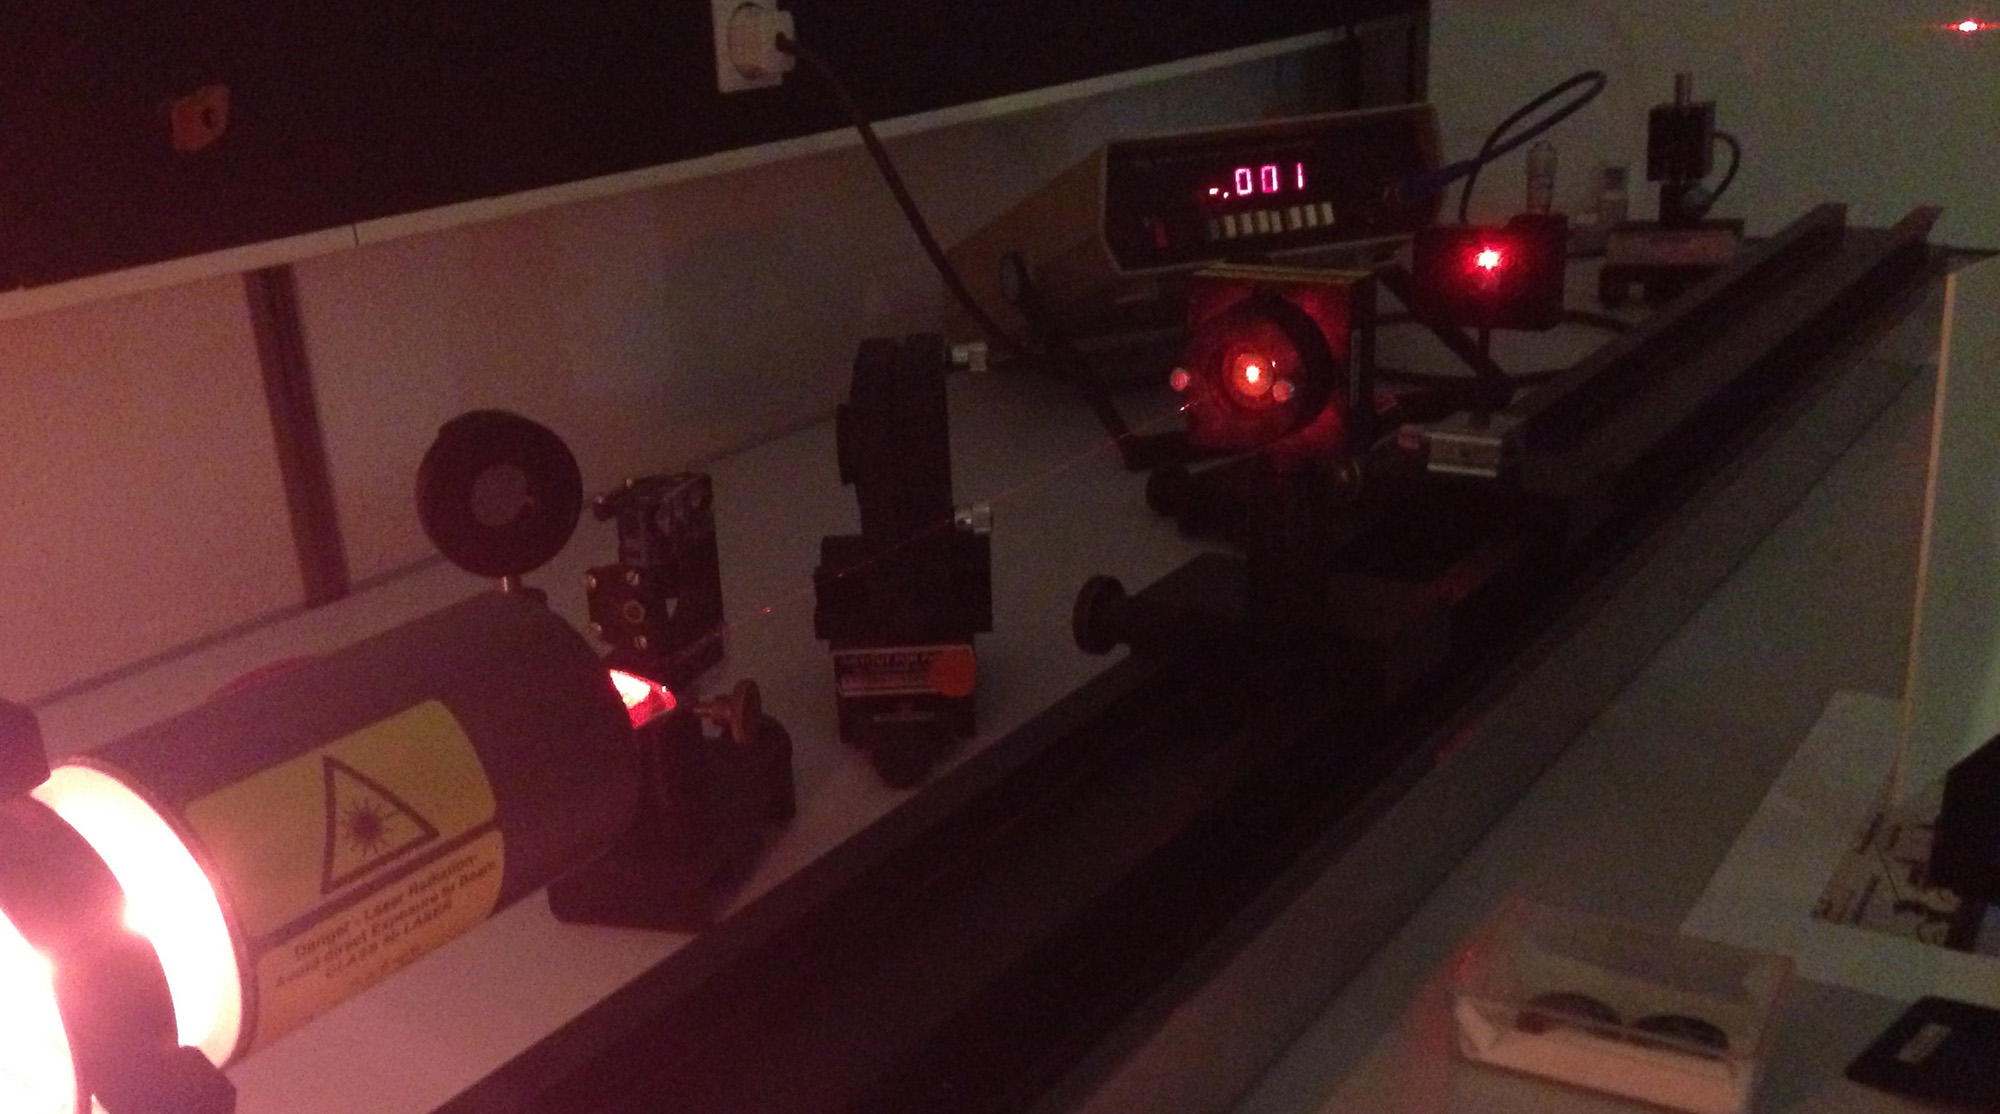
\includegraphics[width=0.9\linewidth]{img/laser.jpg}
    \caption{Funktionierender HeNe-Laser.}
    \label{fig:laser}
\end{figure}

\subsection{Untersuchung von TEM-Moden}
\label{subsec:moden}
Zunächst wird nach Funktion des Lasers die $\text{TEM}_{00}$-Mode vermessen.
Um den Intesitätsverlauf auf einem Schirm besser zu erkennen, wird eine Vergrößerungslinse in den Strahlgang eingebracht.
Dafür wird eine Photodiode im Abstand von \SI{80}{\centi\meter} senkrecht zum Strahl verschoben und die Intesität aufgenommen.
Die Messwerte sind in Tabelle \ref{tab:tem00} aufgeführt. In Abbildung \ref{fig:tem00} ist ein Fit einer Gaußfunktion $I_{00}(x)$ aufgetragen, wobei gilt
\begin{equation}
    \label{eqn:gauss}
    I_{00}(x) = I_0 \exp\left[-2 \frac{\left(x-x_0\right)^2}{\omega^2}\right]\,.
\end{equation}
Der Fit liefert für die Verschiebung \input{build/tem00_x.tex}\unskip, die Maximalintensität \input{build/tem00_i.tex} und für den Strahlradius \input{build/tem00_omega.tex}\unskip.
Die Fehler der Messwerte werden mit \SI{5}{\percent} abgeschätzt.
\begin{table}
    \centering
    \caption{Messwerte zur $\text{TEM}_{00}$-Mode.}
    \label{tab:tem00}
    \begin{tabular}{S[table-format=1.1] 
                    S[table-format=1.3]@{$\qquad$}
                    S[table-format=1.1] 
                    S[table-format=1.3]@{$\qquad$}
                    S[table-format=1.1] 
                    S[table-format=1.3]}
        \toprule
        {$x/\si{\milli\meter}$} & {I/\si{\milli\ampere}} &
        {$x/\si{\milli\meter}$} & {I/\si{\milli\ampere}} &
        {$x/\si{\milli\meter}$} & {I/\si{\milli\ampere}} \\
        \midrule
        3.0	& 0.010 & 4.2	& 0.575 & 5.4	& 0.190 \\
        3.2	& 0.026 & 4.4	& 0.744 & 5.6	& 0.118 \\
        3.4	& 0.066 & 4.6	& 0.766 & 5.8	& 0.031 \\
        3.6	& 0.124 & 4.8	& 0.680 & 6.0	& 0.011 \\
        3.8	& 0.238 & 5.0	& 0.555 & 6.2	& 0.002 \\
        4.0	& 0.440 & 5.2	& 0.335 &       & \\
        \bottomrule 
    \end{tabular}
\end{table}
\begin{figure}
    \centering
    \includegraphics[width=0.9\linewidth]{build/TEM_00.pdf}
    \caption{Fit einer Gaußfunktion durch die Messpunkte der $\text{TEM}_{00}$-Mode des HeNe-Lasers.}
    \label{fig:tem00}
\end{figure}
Anschließend wird ein dünner Draht in den Resonator eingebracht und so verschoben, dass auf dem Schirm die $\text{TEM}_{01}$-Mode zu erkennen ist.
Es wird wieder die Intensität gemessen und der Abstand zum Schirm beträgt nun $Z = \SI{76}{\centi\meter}$.
Die Messwerte sind in Tabelle \ref{tab:tem01} aufgeführt und der Fit in Abbildung \ref{fig:tem01} dargestellt.
Als Funktion wird hierbei
\begin{equation}
    \label{eqn:tem01}
    I_{01}(x) = I_0 \left(\frac{x-x_0}{\omega}\right)^2 \exp \left[-2 \frac{\left(x-x_0\right)^2}{\omega^2}\right]
\end{equation}
genutzt \cite{Wiki_TEM}.
Der Fit liefert hierbei \input{build/tem01_x.tex}\unskip, \input{build/tem01_i.tex} und \input{build/tem01_omega.tex}\unskip.
In den Messwerten ist eine Abweichung der Peakhöhen zu erkennen, die möglicherweise auf Neigung der Photodiode zurückzuführen ist.
Auch hier werden die Fehler mit \SI{5}{\percent} abgeschätzt.
\begin{table}
    \centering
    \caption{Messwerte zur $\text{TEM}_{01}$-Mode.}
    \label{tab:tem01}
    \begin{tabular}{S[table-format=2.1] 
                    S[table-format=1.3]@{$\qquad$}
                    S[table-format=2.1] 
                    S[table-format=1.3]@{$\qquad$}
                    S[table-format=2.1] 
                    S[table-format=1.3]@{$\qquad$}
                    S[table-format=2.1] 
                    S[table-format=1.3]}
        \toprule
        {$x/\si{\milli\meter}$} & {I/\si{\milli\ampere}} &
        {$x/\si{\milli\meter}$} & {I/\si{\milli\ampere}} &
        {$x/\si{\milli\meter}$} & {I/\si{\milli\ampere}} &
        {$x/\si{\milli\meter}$} & {I/\si{\milli\ampere}} \\
        \midrule
        31.0 & 0.031 & 23.2 & 0.250 & 15.4 & 0.090 & 7.6  & 0.140 \\
        30.8 & 0.034 & 23.0 & 0.280 & 15.2 & 0.110 & 7.4  & 0.140 \\
        30.6 & 0.035 & 22.8 & 0.260 & 15.0 & 0.130 & 7.2  & 0.130 \\
        30.4 & 0.037 & 22.6 & 0.240 & 14.8 & 0.130 & 7.0  & 0.130 \\
        30.2 & 0.038 & 22.4 & 0.250 & 14.6 & 0.160 & 6.8  & 0.100 \\
        30.0 & 0.040 & 22.2 & 0.235 & 14.4 & 0.150 & 6.6  & 0.093 \\
        29.8 & 0.050 & 22.0 & 0.260 & 14.2 & 0.170 & 6.4  & 0.090 \\
        29.6 & 0.047 & 21.8 & 0.260 & 14.0 & 0.200 & 6.2  & 0.080 \\
        29.4 & 0.060 & 21.6 & 0.240 & 13.8 & 0.210 & 6.0  & 0.075 \\
        29.2 & 0.070 & 21.4 & 0.200 & 13.6 & 0.250 & 5.8  & 0.070 \\
        29.0 & 0.070 & 21.2 & 0.180 & 13.4 & 0.260 & 5.6  & 0.075 \\
        28.8 & 0.072 & 21.0 & 0.170 & 13.2 & 0.280 & 5.4  & 0.080 \\
        28.6 & 0.085 & 20.8 & 0.160 & 13.0 & 0.250 & 5.2  & 0.070 \\
        28.4 & 0.090 & 20.6 & 0.140 & 12.8 & 0.300 & 5.0  & 0.060 \\
        28.2 & 0.108 & 20.4 & 0.130 & 12.6 & 0.350 & 4.8  & 0.055 \\
        28.0 & 0.110 & 20.2 & 0.110 & 12.4 & 0.370 & 4.6  & 0.050 \\
        27.8 & 0.113 & 20.0 & 0.090 & 12.2 & 0.390 & 4.4  & 0.050 \\
        27.6 & 0.140 & 19.8 & 0.095 & 12.0 & 0.300 & 4.2  & 0.045 \\
        27.4 & 0.150 & 19.6 & 0.100 & 11.8 & 0.330 & 4.0  & 0.035 \\
        27.2 & 0.133 & 19.4 & 0.080 & 11.6 & 0.320 & 3.8  & 0.030 \\
        27.0 & 0.156 & 19.2 & 0.080 & 11.4 & 0.320 & 3.6  & 0.033 \\
        26.8 & 0.170 & 19.0 & 0.060 & 11.2 & 0.300 & 3.4  & 0.026 \\
        26.6 & 0.180 & 18.8 & 0.060 & 11.0 & 0.293 & 3.2  & 0.021 \\
        26.4 & 0.170 & 18.6 & 0.034 & 10.8 & 0.340 & 3.0  & 0.023 \\
        26.2 & 0.183 & 18.4 & 0.031 & 10.6 & 0.300 & 2.8  & 0.024 \\
        26.0 & 0.195 & 18.2 & 0.032 & 10.4 & 0.310 & 2.6  & 0.019 \\
        25.8 & 0.200 & 18.0 & 0.020 & 10.2 & 0.320 & 2.4  & 0.018 \\
        25.6 & 0.199 & 17.8 & 0.014 & 10.0 & 0.260 & 2.2  & 0.015 \\
        25.4 & 0.210 & 17.6 & 0.009 & 9.8  & 0.250 & 2.0  & 0.012 \\
        25.2 & 0.220 & 17.4 & 0.009 & 9.6  & 0.240 & 1.8  & 0.013 \\
        25.0 & 0.250 & 17.2 & 0.010 & 9.4  & 0.240 & 1.6  & 0.008 \\
        24.8 & 0.260 & 17.0 & 0.013 & 9.2  & 0.230 & 1.4  & 0.007 \\
        24.6 & 0.270 & 16.8 & 0.015 & 9.0  & 0.220 & 1.2  & 0.005 \\
        24.4 & 0.285 & 16.6 & 0.023 & 8.8  & 0.210 & 1.0  & 0.004 \\
        24.2 & 0.300 & 16.4 & 0.035 & 8.6  & 0.200 & 0.8  & 0.004 \\
        24.0 & 0.300 & 16.2 & 0.039 & 8.4  & 0.200 & 0.6  & 0.003 \\
        23.8 & 0.310 & 16.0 & 0.050 & 8.2  & 0.190 & 0.4  & 0.003 \\
        23.6 & 0.300 & 15.8 & 0.060 & 8.0  & 0.190 & 0.2  & 0.002 \\
        23.4 & 0.260 & 15.6 & 0.080 & 7.8  & 0.200 & 0.0  & 0.001 \\
        \bottomrule 
    \end{tabular}
\end{table}
\begin{figure}
    \centering
    \includegraphics[width=0.9\linewidth]{build/TEM_01.pdf}
    \caption{Fit der Funktion \eqref{eqn:tem01} durch die Messpunkte der $\text{TEM}_{01}$-Mode des HeNe-Lasers.}
    \label{fig:tem01}
\end{figure}

\subsection{Polarisationsmessung}
\label{subsec:polarisation}
Mit Hilfe eines Polarisators wird die Polarisationsrichtung des Laserstrahls  
vermessen.
Dazu wird die Intensität des Lichts in Abhängigkeit zur Drehung des
Polarisators gemessen.
Diese sollte einer Sinuskurve mit Amplitude $I_0$ und Offset $\varphi$ folgen:
\begin{equation*}
    I(\theta) = I_0 \sin^2\!\left(\theta-\varphi\right)\,.
\end{equation*}
Die für den Fit genutzten Messwerte sind in Tabelle \ref{tab:polarisation}
aufgeführt. Abbildungen \ref{fig:polarisation} und \ref{fig:polarisation_polar}
Zeigen den Intensitätsverlauf.
Der Fit liefert \input{build/polarisation_I0.tex} und
\input{build/polarisation_phi.tex}\unskip.
\begin{figure}
    \centering
    \includegraphics[width=0.9\linewidth]{build/polarisation_lin.pdf}
    \caption{Intensitätsverlauf hinter Polarisator.}
    \label{fig:polarisation}
\end{figure}
\begin{figure}
    \centering
    \includegraphics[width=0.9\linewidth]{build/polarisation_polar.pdf}
    \caption{Intensitätsverlauf hinter Polarisator -- Polar dargestellt.}
    \label{fig:polarisation_polar}
\end{figure}
\begin{table}
    \centering
    \caption{Messwerte zur Polarisationsmessung des Lasers.}
    \label{tab:polarisation}
    \input{build/polarisation_tab.tex}
\end{table}

\subsection{Wellenlängenbestimmung}
\label{subsec:wellenlänge}
Mit einer Vermessung verschiedener Beugungsmuster wird nun die Wellenlänge des
Lasers bestimmt.
Dabei wird zunächst ein Spalt mit der Breite $s = \SI{0.5}{\milli\meter}$ in den Lichtweg eingebracht.
Anschließend werden mit Hilfe der Photodiode die Positionen $x_i$ der Minima des Musters ermittelt.
Der Abstand zwischen Spalt und Ebene der Photodiode beträgt $d = \SI{64.5}{\centi\meter}$.
Die Messwerte sind in Tabelle \ref{tab:spalt} aufgeführt und ergeben mit der Beziehung
\begin{equation}
    \label{eq:spalt}
    \lambda_n = \frac{s}{n}\sin\!\left(\alpha_n\right) = \frac{s}{n}\sin\!\left(\arctan\frac{x_n}{d}\right)
\end{equation}
den Mittelwert \input{build/lambda_slot.tex}\unskip.
Hierbei bezeichnet $\alpha$ den Winkel, unter dem das Minimum einfällt.

Zusätzlich wird die Wellenlänge durch Austausch des Spaltes gegen ein Gitter mit Gitterkonstante $g = \SI{10}{\micro\meter}$ bestimmt.
Statt der Minima werden hier die Hauptmaxima des Beugungsmusters vermessen und die Wellenlänge mit
\begin{equation}
\label{eq:gitter}
    \lambda_n = \frac{g}{n}\sin\!\left(\arctan\frac{x_n}{d}\right)
\end{equation}
bestimmt.
Bei einem Durchgang wird dabei die Photodiode im Abstand von $d = \SI{13.2}{\centi\meter}$ zur Detektion der Maxima genutzt während bei einem zweiten Durchgang die Maxima auf einem Schirm im Abstand von $d = \SI{98}{\centi\meter}$ ausgemessen werden.
Die entsprechenden Messwerte sind in Tabelle \ref{tab:grid} aufgeführt und liefern \input{build/lambda_grid.tex}\unskip.
% Bei allen mit der Photodiode aufgenommenen Messwerten wurde jeweils die Mittelposition $x_0$ bestimmt und abgezogen.
% Diese betrug für den Spalt $x_{0,\text{Spalt}}=\SI{5.8}{\milli\meter}$ und für das Gitter $x_{0,\text{gitter}}=\SI{5.0}{\milli\meter}$.
\begin{table}
    \centering
    \caption{Messwerte, aufgenommen mit Hilfe eines optischen Spaltes.}
    \label{tab:spalt}
    \begin{subtable}{0.49\linewidth}
        \centering
        \caption{Linke Messwerte}
        \label{tab:spalt_links}
        \input{build/lambdas_slot_mm_l.tex}
    \end{subtable}
    \begin{subtable}{0.49\linewidth}
        \centering
        \caption{Rechte Messwerte}
        \label{tab:spalt_rechts}
        \input{build/lambdas_slot_mm_r.tex}
    \end{subtable}
\end{table}
\begin{table}
    \centering
    \caption{
        Messwerte, aufgenommen mit Hilfe eines optischen Gitters.
        Die Werte in \ref{tab:grid_gross} wurde dabei mit Hilfe eines
        Maßbandes in großem Abstand vom Gitter genommen, während die übrigen
        Werte mit Hilfe der Photodiode in geringerem Abstand vom Gitter
        aufgenommen wurde.
    }
    \label{tab:grid}
    \begin{subtable}[t]{0.32\linewidth}
        \centering
        \caption{Großer Aufbau.}
        \label{tab:grid_gross}
        \input{build/lambdas_grid_cm.tex}
    \end{subtable}
    \begin{subtable}[t]{0.32\linewidth}
        \centering
        \caption{Kleiner Aufbau, links.}
        \label{tab:grid_links}
        \input{build/lambdas_grid_mm_l.tex}
    \end{subtable}
    \begin{subtable}[t]{0.32\linewidth}
        \centering
        \caption{Kleiner Aufbau, rechts.}
        \label{tab:grid_rechts}
        \input{build/lambdas_grid_mm_r.tex}
    \end{subtable}
\end{table}

\subsection{Überprüfung der Stabilitätsbedingungen}
\label{subsec:stabilitätsbedingungen}
Zur Prüfung der Stabilitätsbedingungen werden die Resonatorspiegel schließlich
langsam auseinandergeschoben.
Dabei erlischt der Laser immer wieder, kann jedoch durch Nachkalibrierung
etliche Male erneut aktiviert werden.
Mit dieser Methode wurde der maximale Abstand $d_\text{max}$,
unter dem der Laser arbeitet
für einen planen Spiegel (Krümmungsradius $r = \infty$) und einen konvexen
Spiegel mit Krümmungsradius $r = \SI{1}{\meter}$ bestimmt.
Nach Gleichung \eqref{eqn:stabi} erlischt der Laser bei beiden Spiegeln nach
$d_\text{max}^\text{theorie} = \SI{1}{\meter}$. Der konvexe Spiegel soll
zusätzlich hinter $d_\text{max}^{\text{theorie}\prime} = \SI{1.4}{\meter}$ eine
Reaktivierung des Lasers ermöglichen.
Die maximalen gemessenen Abstände betragen:
\begin{align*}
    d_\text{max,plan} = \SI{80\pm0.5}{\centi\meter} \qquad
    d_\text{max,konvex} = \SI{98\pm0.5}{\centi\meter}\,.
\end{align*}
Bei dem konvexen Spiegel gelingt es in einem Abstand von
$d=\SI{142\pm0.5}{\centi\meter}$ den Laser zu reaktivieren, wobei dieser Aufbau
auf kleinste Stöße am Tisch reagiert und der Laser erlischt.

\subsection{Gaußverbreiterung beim HeNe-Laser}
\label{subsec:gauß_diskussion}
Die in \ref{subsec:gaußverbreiterung} beschriebene Gaußverbreiterung wird im
Folgenden exemplarisch behandelt.
Es wird geklärt, wie viele Schwingungsmoden in diesem Profil erhalten sind.
Um die Breite des Gaußprofiles zu bestimmen, wird die Temperatur mit 
$T = \SI{300}{\kelvin}$ geschätzt. Die Frequenz des Lasers beträgt etwa
$f_0 = \SI{500}{\tera\hertz}$ und die Molekülmasse wird mit einigen
Protonmassen genähert.
Damit ergibt sich eine Breite des Gaußprofiles von $\sigma_f \
\approx \SI{0.5}{\giga\hertz}$.

Für eine Resonanz muss die Wellenlänge der Strahlung zudem einem Vielfachen
der Resonatorlänge $L\approx \SI{1.5}{\meter}$ entsprechen, woraus folgt, dass
\begin{equation*}
    f_n = n \frac{\mathrm{c}}{2L}\,.
\end{equation*}
Der Abstand $\Delta f_n$ der einzelnen Schwingungsmoden beträgt damit 
$\Delta f_n \approx \SI{100}{\mega\hertz}$.

Als Richtwert für die Zahl der enthaltenen Moden im Spektrum wird das
Verhältnis von Modenabstand $\Delta f_n$ und Halbwertsbreite des Gaußprofiles
$2\sqrt{2\ln2} \sigma_f$ gebildet.
Nach dieser Abschätzung enthält das Spektrum etwa \num{10} Schwingungsmoden
des Lasers.
Abbildung \ref{fig:gauß} veranschaulicht diesen Effekt.
\begin{figure}
    \centering
    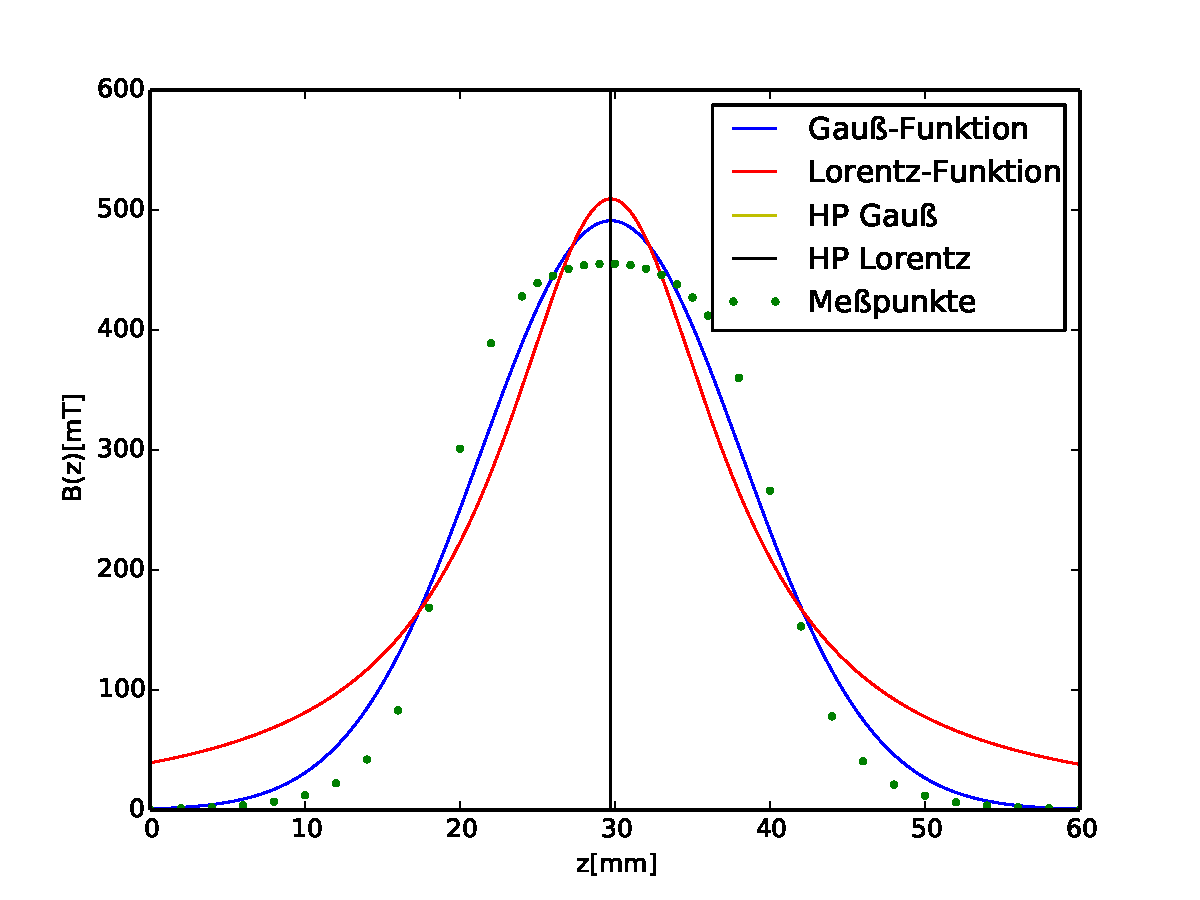
\includegraphics[width=0.9\linewidth]{build/gauss.pdf}
    \caption{
        Veranschaulichung des Gaußprofiles und der natürlichen Linienbreite
        des HeNe-Lasers.
    }
    \label{fig:gauß}
\end{figure}
